\documentclass[12pt, a4paper, oneside, romanian]{teza-upb}
\setcounter{secnumdepth}{3}
\setcounter{tocdepth}{3}
\usepackage{babel}
\usepackage{graphicx}
\usepackage{float}
\usepackage[
  bookmarksnumbered,
  bookmarks,
  bookmarksopen=true,
  pdftitle={Dizertatie},
  linktocpage]{hyperref}
\singlespacing
\begin{document}
\begin{titlepage}
	\centering
	
\includegraphics[width=0.15\textwidth]{img/UPB-logo.png}\par\vspace{1cm}
	{\scshape\LARGE Facultatea de Electronică, Telecomunicații și Tehnologia Informației \par}
	\vspace{1cm}
	{\huge Sesiunea de comunicări sțiințifice\par}
	{\large 2016 \par}
	\vspace{1cm}
	{\huge\bfseries Arhitecturi pentru sisteme auto-scalabile: microservicii\par}
	\vspace{2cm}
	{\Large\bfseries Andrei Mihăescu\par}
	\vspace{2cm}
	{\Large\bfseries Conducători științifici: \par}
	{\Large Conf. dr. ing. Eduard-Cristian POPOVICI \par}
	{\Large Ș.l. dr. ing. Radu BADEA\par}
% Bottom of the page
\end{titlepage}
\newpage

\chapter{Motivație}

Datorită avansurilor tehnologice uriașe în domeniul informaticii și al telecomunicațiilor astăzi, mai mult ca niciodată, o foarte mare parte a activităților coditiene (fie ele profesionale sau personale) sunt stâns legate de domeniul virtual. Revoluția digitală a schimbat complet modul în care folosim sistemele informatice, care acum stau la baza foarte multor afaceri din toate domeniile (plecând de la cel bancar și terminând cu cel agricol) în proporție de 24\% cu previziuni ca această cifra să se dubleze până în 2020 - \textit{"Forrester Research - The State of Digital Business, 2015 to 2020"}.

Această expansiune a pus o presiune enormă asupră inginerilor din domeniul informatic, care se confruntă cu o adevărată provocare pentru a crea sisteme robuste capabile să satisfacă această nevoie crescândă. Pornind de la această nevoie, conceptul de aplicație de tip "enterprise" a luat naștere. O astfel de aplicație trebuie să răspundă anumitor standarde și cerințe pentru a putea asigura buna funcționare a unei afaceri:
\begin{itemize}
 \item \textbf{flexibilitate} - o aplicație bine gândită trebuiă să permită modificări, ce apar ca urmarea a evoluției domeniului în care este folosită; aceastea trebuie ușor implementate, pentru a crea valoare pentru utilizatori.
 \item \textbf{robustețe} - în proiectarea unei aplicații trebuie luate în calcul cât mai multe cazuri în care aceasta ar putea fi exploatată și compromisă, creând astfel întreruperi în funizarea serviciilor.
 \item \textbf{scalabilitate} - având in vedere dorința fiecărei afaceri de a prospera și a crește este de așteptat ca și aplicațiile folosite să se poată adapta la volume din ce în ce mai mari de procesări. 
 \item \textbf{securitate} - dat fiind faptul că o aplicație poate deveni principala sursă de venit din cadrul unei companii este nevoie ca aceasta să respecte cel mai înalte standarde de securitate astfel încât datele utilizatorilor să fie bine protejate. 
\end{itemize}

Pentru a răspunde tuturor acestor nevoii, un sistem informatic trebuie să fie slab cuplat (eng. \textit{loosely-coupled}), pentru a asigura flexibilitate, să aibă mecanisme ce asigură redundanța, pentru robustețe, să aibă un grad mare de modularizare pentru a fi scalabil și să implementeze principiul eng. \textit{AAA - Authentication, Authorization \& Accounting} pentru a fi sigur.


\chapter{Aplicații monolit}

Aplicațiile \textbf{monolit} reprezintă modul tradițional de dezvoltarea a unei aplicații, fie ea chiar și de tip enteprise. În cadrul aplicațiilor monolit toată funcționalitatea este dezvoltată în cadrul unui artefact care este livrat la final și trimis în producție. Acest model prezintă o serie de avantaje și dezavantaje. 

Printre primele avantaje ale acest tip de aplicație se numără faptul că este ușor de dezvoltat; din punct de vedere arhitectural nu implică eforturi mari. Totul este dezvoltat ca un singur bloc a cărui componente pot fi organizate pe module, însă sunt reunite și livrate sub forma unui singur produs final. În mod tipic o astfel de aplicație va rula pe unul sau mai multe servere. Fiecare dintre acestea fiind identic toate componentele din cadrul aplicație vor comunica între ele la nivel de proces, fără a implica vreun fel de comunicare cu exteriul, exceptând prin intermediul punctelor terminale (\textit{eng. end point}) special construite. Acest tip de aplicație prezintă un grad relativ scăzut de complexitate, aceasta din punct de vedere arhitectural, deoarece complexitatea logici de business nu este corelată cu arhitectura aplicației. Mentenanța unei astfel de aplicații este facilă, întreg codul situându-se într-un singur loc, procesul de depanare se poate desfăsura ușor. 

În ciuda acestor avantaje care ar putea înclină balanța în favoarea aplicațiilor monolit,ele prezintă o serie de dezavantaje care îngreunează procesul de creare de valoare prin implementarea nevoilor unei afaceri. Faptul că toate componentele sunt în cadrul unui singur artefact determină un nivel înalt de cuplare între acestea - \textit{eng. tightly coupled} - ceea ce duce la o scădere a flexibilității și deci o reducere a ritmului de implementare a schimbărilor. Legat de acest fapt este randamentul slab în ceea ce privește scalabilitatea. Aplicația nu poate scala decât cu o granularitate de o instanță, nu de un modul al său de care poate fi nevoie. Astfel spus, pentru a îmbunătații performanța unui modul toată aplicație trebuie instalată pentru un alt server. Un dezavantaj, ar fi legat de modul de instalare a aplicațiilor pe diverse medii (dezvoltare, testare sau producție). Adesea o nouă instalare (\textit{eng. deploy}) vizează o singură componentă, însă pentru a livra schimbarea toată aplicația trebuie recompilată și instalată.

Deși avantajele acestor aplicații nu sunt de neglijat, ele prezintă dezavantaje care le fac să nu mai fie relevante în contextul actual al tendințelor, care orientate pe flexibilitate și pe livrarea în producție cât mai rapidă a produselor informatice. 

\chapter{Aplicații bazate pe microservicii}

Aplicațiile bazate pe microservicii fac parte dintr-o categorie mai largă de aplicații care sunt înscriu în capitolul aplicațiilor orientate pe servicii (\textit{eng. SOA - Service Oriented Architecture}). Caracteristicile arhitecturii SOA sunt:
\begin{itemize}
 \item Serviciile sunt autonome. Fiecare serviciu este menținut, dezvoltat, instalat și versionat în mod independent.
 \item Serviciile pot fi distribuite. Serviciile pot fi localizate oriunde pe rețea, local sau la distanță, atât timp cat rețeaua dispune de protocoalele necesare de comunicare.
 \item Serviciile sunt slab cuplate. Fiecare serviciu este independent față de celălalte și poate fi înlocuit și actualizat fără a întrerupe celălalte aplicații care îl folosesc atât timp cât interfețele sunt compatibile.
 \item Serviciile împart schema și contractul, nu clasa. Serviciile partajează contracte și scheme atunci când comunică, și nu clase interne.
\end{itemize}

\begin{figure}[ht]
\centering
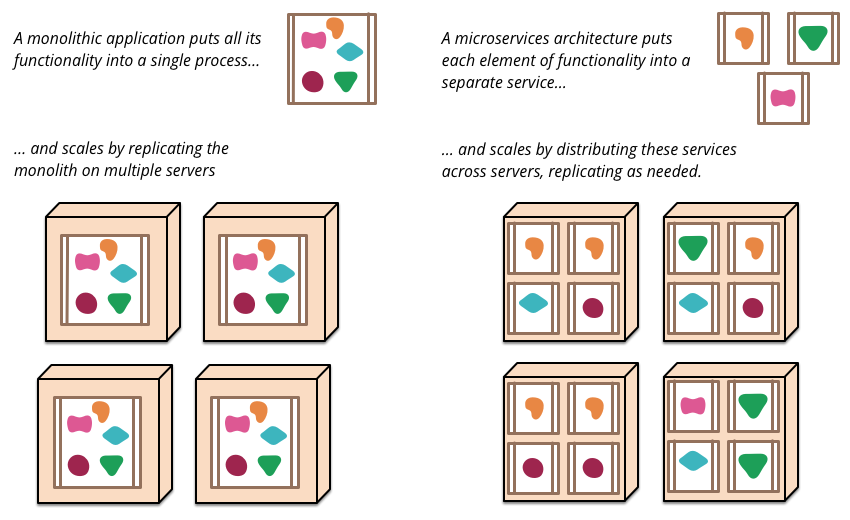
\includegraphics[scale=0.3]{img/sketch.png}
\caption{Aplicații monolit și aplicații bazate pe microservicii}
\label{fig:arhi_mono_micro}
\end{figure}

Plecând de la aceste caracteristici ideea microserviciilor duce mai departe distribuirea și slaba cuplare a serviciilor, astfel că dezvoltarea unuei aplicații este realizată ca o suită de mici servicii, fiecare rulând un proces independent și comunicând prin mecanisme simple, adesea resurse expuse prin API-uri via HTTP. Pe lângă faptul ca serviciile pot fi instalate și scalate în mod independent, fiecare crează o limită fermă a modulului, permițând chiar și folosirea limbajelor de programare diferite, acestea putând fii gestionate de echipe diferite.




\end{document}